% @Author: WU Zihan
% @Date:   2022-05-04 12:24:46
% @Last Modified by:   WU Zihan
% @Last Modified time: 2022-05-04 12:36:19
\documentclass[aspectratio=169]{beamer}
\usepackage{graphicx}
\usepackage{amssymb,amsfonts,amsmath}
\usepackage{tikz,tkz-euclide}
\usepackage{subfigure}
\usepackage{parskip}
\usetikzlibrary{arrows.meta}
\usetikzlibrary{calc,patterns}
\usefonttheme[onlymath]{serif}
% \usetheme{Berlin}
\title{Detection of 3D circles / Ellipses in a photo}
\author{WU Zihan}
\subtitle{Supervisor: Prof. YAN Hong}
\begin{document}
\setbeamertemplate{background}
{
\includegraphics[width=\paperwidth]{EE8001 Presentation Template.pdf}} 
    \maketitle
    \section{Target}
    \begin{frame}
        \frametitle{Project Target}
    
        To detect ellipses in the images/videos.
        \begin{columns}
            \begin{column}{.5\linewidth}
                \begin{figure}
                    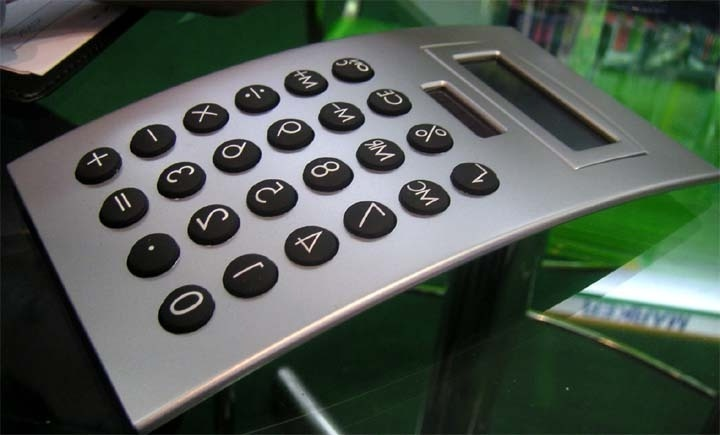
\includegraphics[width=0.8\linewidth]{pic/source.jpg}
                    \caption{Input}
                \end{figure}
            \end{column}
            \begin{column}{.5\linewidth}
                \begin{figure}
                    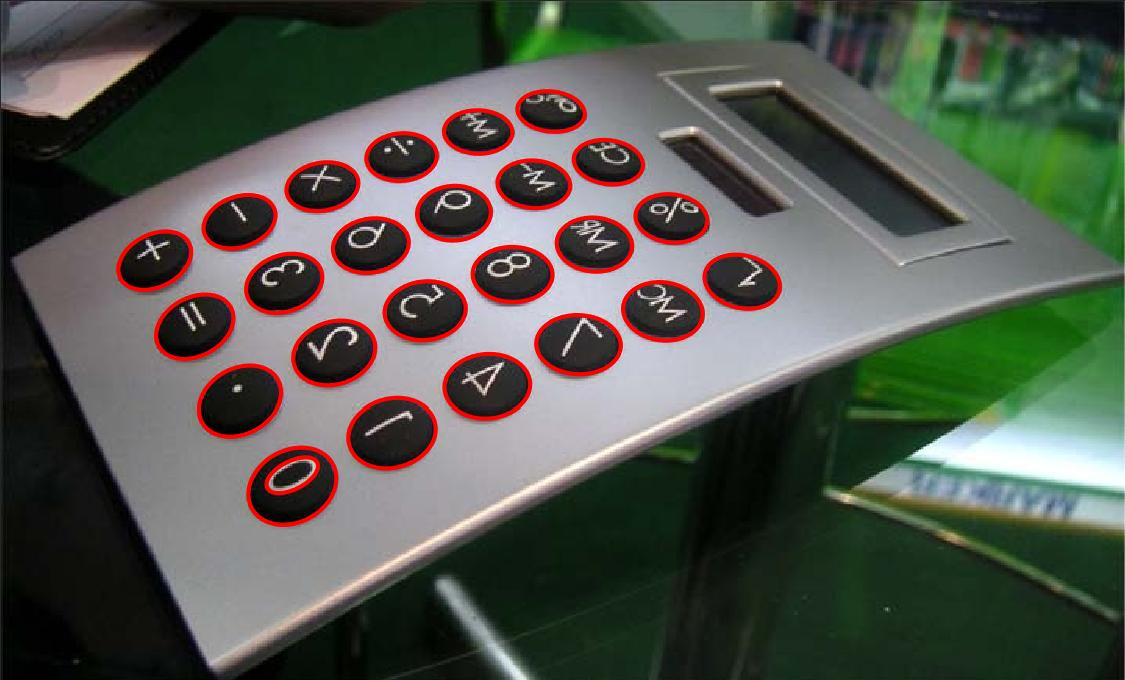
\includegraphics[width=0.8\linewidth]{pic/ideaoutput.jpg}
                    \caption{Output}
                \end{figure}
            \end{column}
        \end{columns}
    
    \end{frame}
    \section{Methods}
    \begin{frame}
        \frametitle{Methods}
    
        \begin{itemize}
            \item To detect the arc segements;
            \item (To form arcs;)
            \item To predict the 5 parameters for ellipses;
            \item Co-clustering;
            \item Validation.
        \end{itemize}
    
    \end{frame}
    \subsection{cocluster}
    \begin{frame}
        \frametitle{Cluster/Co-cocluster}

        \begin{figure}
            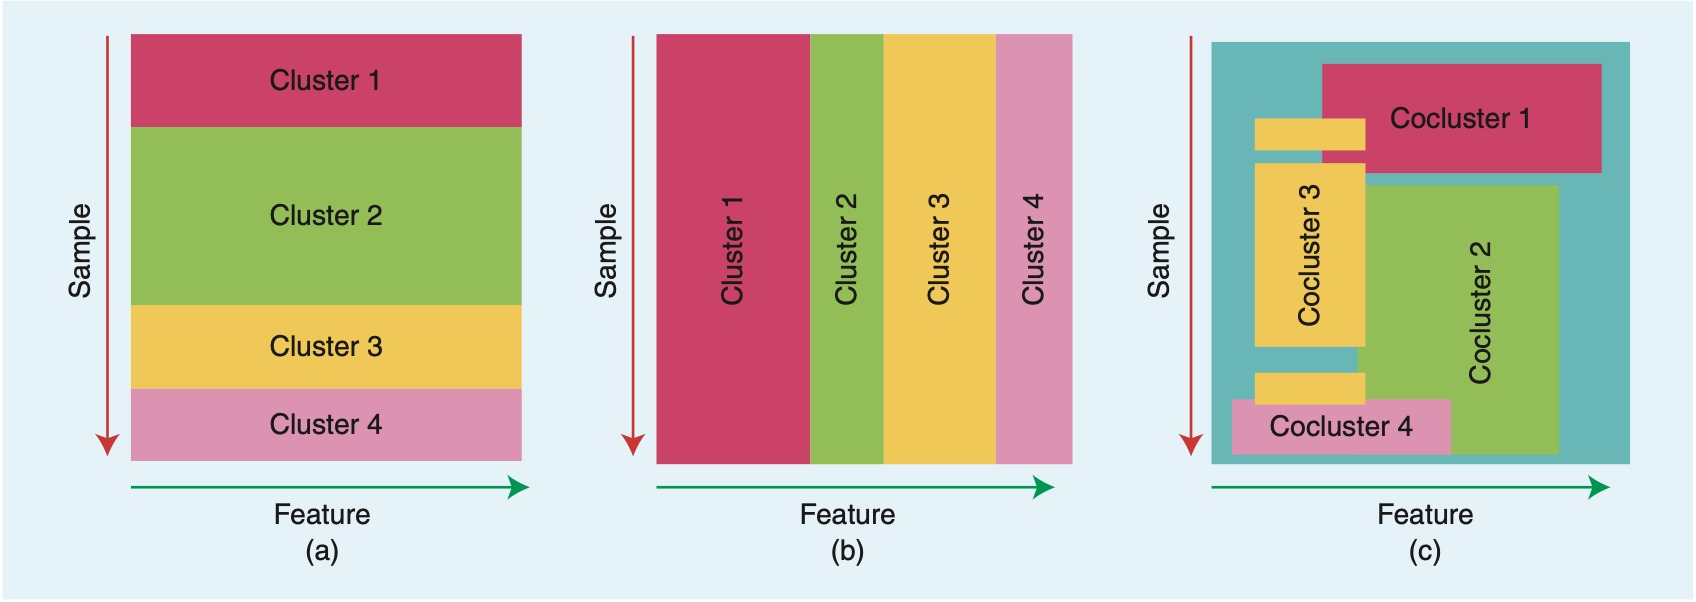
\includegraphics[width=0.8\linewidth]{pic/cocluster.png}
            \caption{cocluster method}
        \end{figure} 
    \end{frame}
    \subsection{Validation}


    \begin{frame}
        \frametitle{Pilot Result}
        \begin{columns}
            \begin{column}{.5\linewidth}
                \begin{figure}[htbp]
                    \centering
                    \subfigure{
                        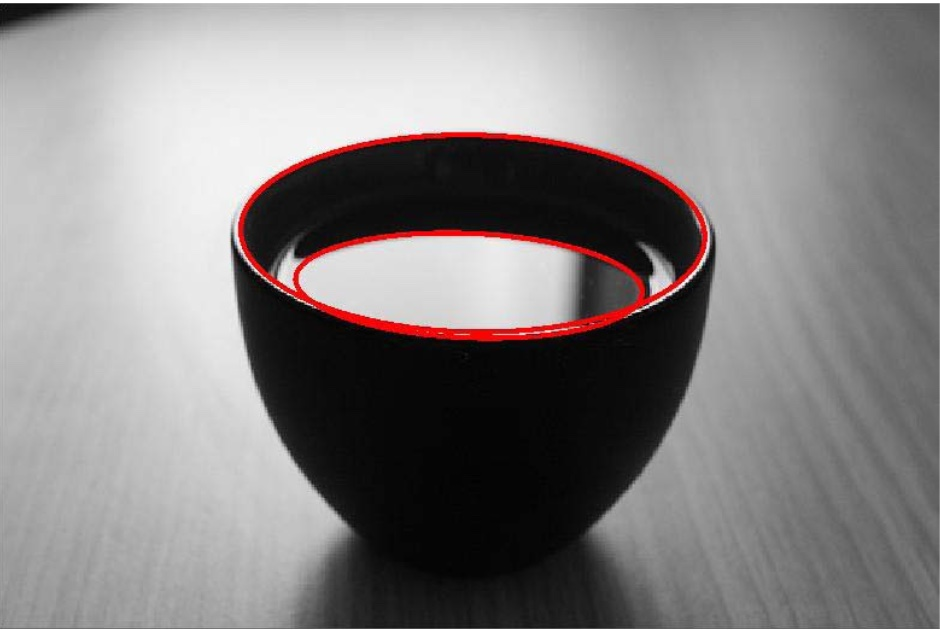
\includegraphics[width=0.7\linewidth]{pic/cup.jpg}
                    }
                    \quad
                    \subfigure{
                        \includegraphics[width=0.7\linewidth]{pic/coin.jpeg}
                    }
                    \caption{Good Examples}
                \end{figure}
            \end{column}
            \begin{column}{.5\linewidth}
                \begin{figure}[htbp]
                    \centering
                    \subfigure{
                        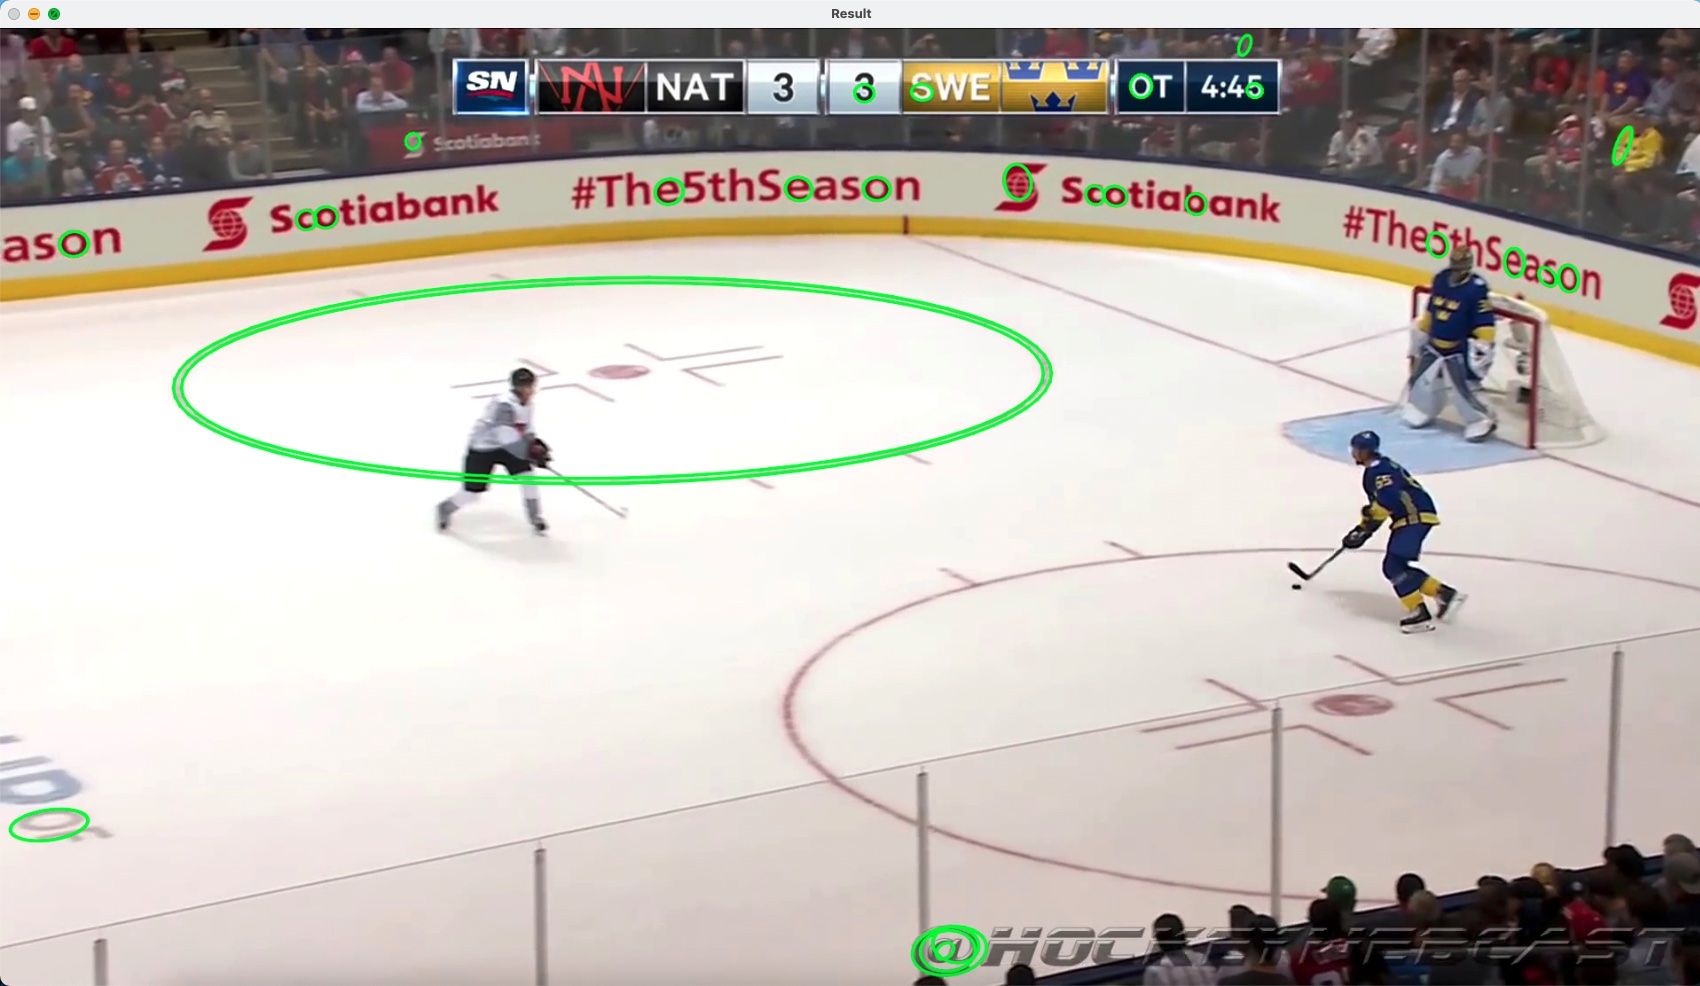
\includegraphics[width=0.7\linewidth]{pic/Hockeyre.jpg}
                    }
                    \quad
                    \subfigure{
                        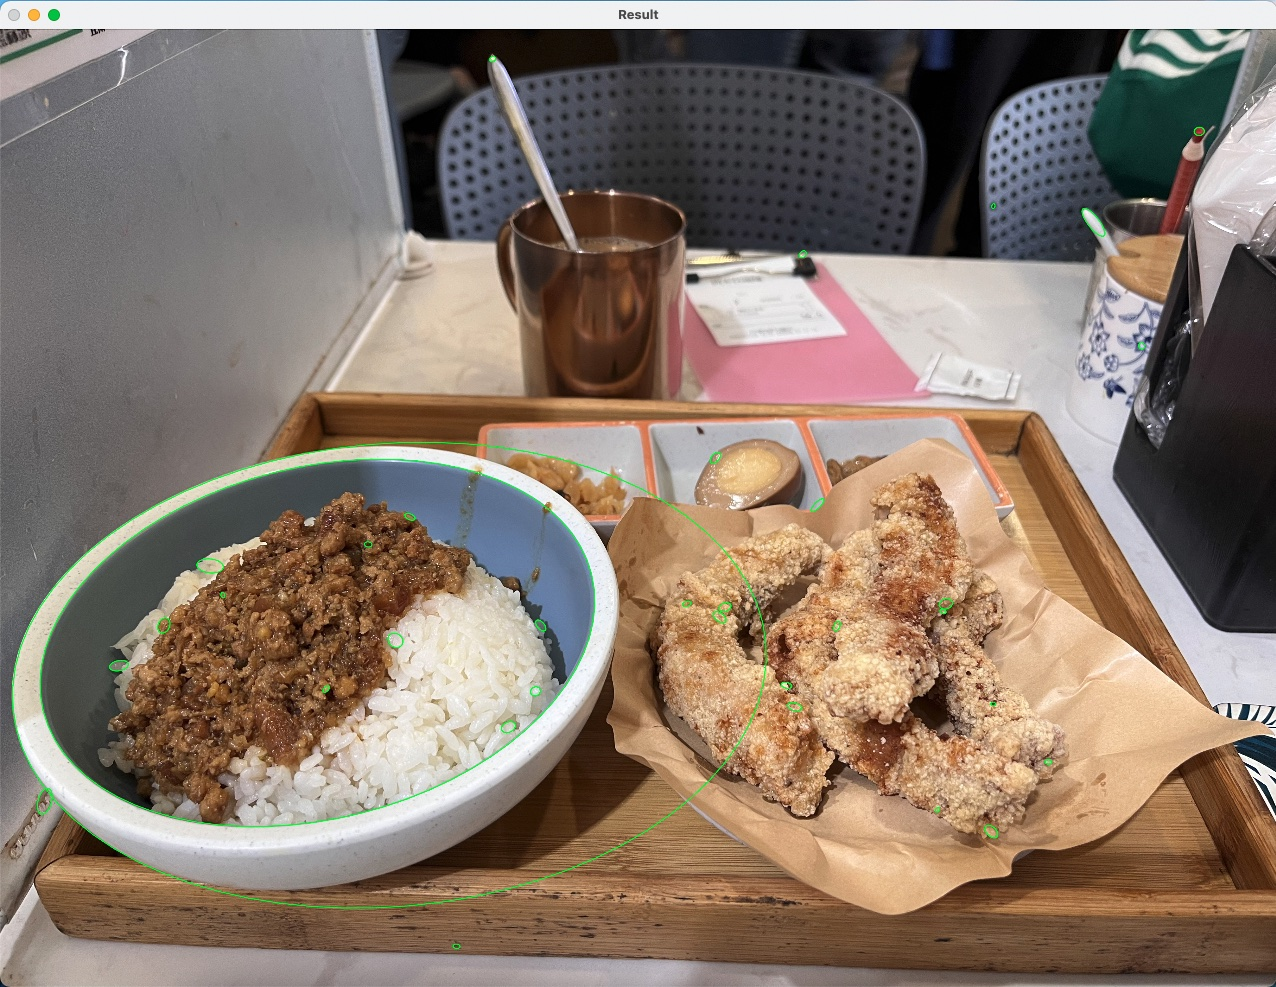
\includegraphics[width=0.7\linewidth]{pic/rice.jpg}
                    }
                    \caption{Bad Examples}
                \end{figure}
            \end{column}
        \end{columns}
        

    \end{frame}



    \begin{frame}
        \frametitle{Summary}
    
        \begin{enumerate}
            \item Co-clustering is effective to grouping data with good accuracy taking ellipses for examples. 
            \item Co-clustering can serve as an unsupervised learning model in grouping problems.
            
        \end{enumerate}
    
    \end{frame}
    \begin{frame}
        \frametitle{Q\&A}
    
        Thank you!
    
    \end{frame}
\end{document}